\section{Grundlagen}\raggedbottom
In diesem Kapitel werden die Grundlagen zu den verwendeten Technologien vorgestellt. 
Zunächst wird die in dieser Masterarbeit untersuchte Aufgabe des abstrakten Zusammenfassens von mehreren Dokumenten erläutert.
Anschließend werden die Grundlagen zu neuronalen Netzen und insbesondere zu Deep Learning zusammengefasst dargestellt. 
Hier wird ebenfalls die Struktur von Sequence-To-Sequence Modellen und LSTM-Zellen erläutert.

Im folgenden Kapitel \ref*{transformer} wird anschließend aus den Grundlagen die verwendete Transformer Architektur, BERT und GPT-2 konkretisiert.


\subsection{Textzusammenfassung}
Das automatisierte Zusammenfassen von Texten ist ein Teilgebiet des NLP, welches sich mit dem Zusammenfassen von langen Texten zu einem kongruenten, kürzeren Text unter Beibehaltung von wichtigen Informationen befasst. 
Durch die zunehmenden Datenmengen wird automatisierte Textzusammenfassung immer relevanter, um akkurat aggregierte Zusammenfassungen und Überblicke zu geben.
Automatisierte Textzusammenfassung lässt sich zum Beispiel bei der Generierung von Kurzzusammenfassungen zu Dokumenten verwenden.

Grundsätzlich wird beim automatisierten Zusammenfassen von Texten zwischen den extraktiven und den abstraktiven Methoden unterschieden.

\subsubsection{Extraktive Textzusammenfassung}
Extraktive Textzusammenfassung ist das Identifizieren und anschließende Extrahieren von wichtigen Phrasen oder Sätzen aus dem Ursprungstext.
Hierbei werden die entsprechend ausgewählten Phrasen in der Zusammenfassung genauso wie sie im Ursprungstext vorkommen übernommen.
Die zu extrahierenden Phrasen oder Sätze werden mithilfe einer Scoringfunktion gefunden und später aneinander gereiht. Hierzu gibt es unterschiedliche Methoden und Metriken.

\subsubsection{Abstraktive Textzusammenfassung}
Abstraktive Textzusammenfassung versucht durch Interpretation und Verständnis des Ursprungtexts eine kurze, kongruente Zusammenfassung zu produzieren. 
Die Zusammenfassung soll alle wichtigen Informationen enthalten und als zusammenhängender flüssiger Text erzeugt werden. Ein kongruenter Text wird erzeugt, da das Sprachmodell frei Sätze produzieren kann und nicht an vorher vorgegebene Sätze oder Phrasen gebunden ist, wie bei der extraktiven Zusammenfassung.

Große Fortschritte im Bereich der abstraktiven Textzusammenfassung ergaben sich in den letzten Jahren durch Sequence-To-Sequence Modelle. Diese encodieren den Eingabetext in eine Übergangsrepresentation und generieren aus dieser durch Decodierung eine Ausgangsrepresentation.

\subsubsection{Multi-Document Textzusammenfassung}
Eine große Herausforderung ist das Zusammenfassen von mehreren Dokumenten über dasselbe Thema zu einem einzigen Dokument. 
Die entstehende Zusammenfassung soll Anwendern einen guten und schnellen Überblick über eine große Anzahl an Dokumenten bieten. 
Die unterschiedlichen Dokumente enthalten diverse Informationen die sich nicht immer im Ergebnis und Vokabular deckungsgleich sind. 
Somit ergibt sich die Herausforderung, unterschiedliche Perspektiven in den jeweiligen Dokumenten zusammenfassend zu representieren.
Da sich unterschiedliche Standpunkte schlecht mittels extraktiven Methoden darstellen lassen, bieten sich bei der Multi-Document Textzusammenfassung die Verwendung abstraktiver Methoden an.
Damit kann eine kongruente Zusammenfassung generiert werden, die die unterschiedlichen Aspekte der Dokumente darstellt.

In dieser Masterarbeit werden unterschiedliche Rezensionen zu Produkten und Dienstleistungen zusammengefasst. 
Insbesondere Rezensionen unterscheiden sich stark in ihren Nutzerperspektiven und können positiv, negativ oder neutral sein und auf sehr spezifische Eigenschaften der entsprechenden Produkte eingehen.
Es ist eine große Herausforderung aus einer Menge aus Produktrezensionen eine repräsentative zusammenfassende Rezension zu produzieren, die klar strukturiert, kongruent, verständlich und Zielgruppenbezüglich die entsprechenden Inhalte wiedergibt.

\subsection{Deep Learning}
Deep Learning ist ein Teilbereich des Machine Learning, bei dem nach dem Vorbild für das menschliche Gehirn neuronale Netze verwendet werden. 
Neuronale Netze werden unter anderem beim Natural Language Processing eingesetzt. 
Die neuronalen Netze bestehen aus mehreren Layern, die sequentiell den Output des vorherigen Layers weiterverarbeiten. 
Das Ziel von Deep Learning ist, durch Training der neuronalen Netze, Repräsentationen beziehungsweise Approximationen für Funktionen in den Daten zu finden.
Zum Trainieren dieser Netze wird oft Backpropagation, ein Verfahren zur Berechnung der Gradienten in neuronalen Netzen und entsprechender Anpassung der Gewichte verwendet.

\subsection{Word Embeddings}
Word Embeddings werden im Natural Language Processing verwendet, um Wörter mit aussagekräftigen Vektoren zu repräsentieren. 
Hochdimensionale Objekte wie Wörter lassen sich mittels Word Embeddings in einen niedrigdimensionalen Raum darstellen und behalten dabei ihre semantischen Relationen bei. 
Auf diesen Vektoren lassen sich unterschiedliche arithmetische Operationen ausführen.

Bekannte kontextunabhängige Word Embedding Verfahren sind zum Beispiel word2vec \citep{word2vec} und GloVe (Global Vectors for Word Representation) \citep{glove}. 
Diese Verfahren berechnen für jedes Wort einen eindeutigen Vektor, der alle unterschiedlichen Eigenschaften dieses Wortes enthält.
Die errechneten Vektoren sind kontextunabhängig und für ein Wort wird stets der gleiche Vektor verwendet. 
Word2vec erlernt die entsprechenden Vektorrepräsentationen mittels eines SkipGram neuronalen Netzes \citep{word2vec} GloVe hingegen über die nicht Nulleinträge einer Co-occurrence Matrix von Wörtern untereinander \citep{glove}. 

Kontextabhängige Verfahren, wie zum Beispiel ELMO \citep{elmo} oder BERT \citep{DBLP:journals/corr/abs-1810-04805}, generieren kontextabhängige Vektoren für Wörter und Berücksichtugen dabei das Umfeld in dem das einzelne Wort auftritt.
Bei diesen Verfahren wird zur Bestimmung eines Word Embeddings der gesamte Satz benötigt, um die erlernten kontextspezifischen Eigenarten für die Einbettung zu berücksichtigen. 

Verfahren wie zum Beispiel BERT nutzen besondere Tokenisierungsmethoden, die es erlauben einzelne Wörter durch mehrere Tokens zu repräsentieren.
Dieses Splittingverfahren von Wörtern in Subtokens ist als WordPiece Verfahren \citep{wordpiece} für BERT und als BytePairEncoding \citep{bytepairencoding} für GPT-2 bekannt. 
Durch das Splitten in Subtokens und Erlernen von Einbettungen für diese lässt sich ein kleineres Wörterbuch erstellen. 
Da sich die Wörter stets in Subtokens zerlegen lassen können Out-of-Vocabulary-Fehler vermieden werden.

\subsection{Sequence-To-Sequence Modelle}
Sequence-To-Sequence Modelle sind eine Gruppe von Deep Leaning Modellen zur Sprachverarbeitung die eine Textsequenz $(x_1,x_2,\ldots,x_n)$ bestehend aus den Tokens $x_i$ in eine andere Textsequenz $(y_1,y_2,\ldots,y_n)$ überführen \citep{DBLP:journals/corr/SutskeverVL14}.
Die Besonderheit bei diesem Modell liegt darin, dass die Länge der Eingabesequenz und der Ausgabesequenz unterschiedlich sein kann.
Die am meisten verwendeten Sequence-To-Sequence Modelle bestehen aus einer Encoder/Decoder Architektur.
Der Encoder und Decoder besteht jeweils aus sequentiellen Rekurrenten Neuronalen Netzen (RNN), die jeweils als Eingabe ein Token und den Hidden-State des vorherigen RNNs erhalten.
Somit summieren sich innerhalb des Encoders die Hidden-States auf und werden abschließend durch einen Hidden-State Vektor repräsentiert, der die Informationen aus der Eingabe enthält.
Der abschließende Hidden-State Vektor lässt sich wie folgt iterativ bestimmen, wobei $f$ für die entsprechende RNN-Zelle und $W$ für die Gewichtsmatrizen steht:
\begin{equation}
    h_t = f(W^{hh}h_{t-1}+W^{hx}x_t)
\end{equation}

Oft werden als RNN-Zellen Long Short Term Memory (LSTM)- oder Gated Recurrent Unit (GRU)-Zellen verwendet.
Der Decoder ist ebenfalls ein RNN, welcher aus dem Hidden-State Vektor des Encoders eine Ausgabesequenz generiert.

Um die Performance von Sequence-To-Sequence Modellen weiter zu optimieren werden in Kapitel \ref{attention} Attention Modelle eingeführt.


\subsection{\textbf{L}ong \textbf{S}hort \textbf{T}erm \textbf{M}emory}
\textbf{L}ong \textbf{S}hort \textbf{T}erm \textbf{M}emory (LSTM) Netze sind eine Untergruppe der Rekurrenten neuronalen Netze (RNN), die es ermöglichen Langzeitbeziehungen in Daten zu erlernen \citep{lstm}.
Rekurrente Neuronale Netze zeichnen sich durch ihre rekurrenten Verbindungen innerhalb desselben Layers aus, wodurch die nächste RNN-Zelle die vorherigen Informationen weiterverarbeiten kann.
Ein häufiges Problem ist das Modellieren von Langzeitbeziehungen mittels RNNs. 
LSTMs sind speziell darauf ausgelegt diese Langzeitbeziehungen abzubilden, indem sie stets einen Zellzustand mit übergeben.
Eine LSTM-Zelle hat nun die Möglichkeit diesen Zellstatus zu manipulieren, indem Informationen hinzugefügt oder gelöscht werden können.
Diese Manipulationen des Zellstatus wird durch drei Gates ermöglicht. 
Erstens dem Forget Gate, welches der Zelle ermöglicht alte Werte zu vergessen.
Zweitens dem Input Gate, welches steuert zu welcher Gewichtung neue Eingabewerte in dem Hidden-State gespeichert werden.
Drittens dem Output Gate, welches steuert welcher Teil des Hidden-States in die folgende Zelle propagiert wird.

Durch die Anpassung des Hidden-States in den einzelnen Zellen können relevante Informationen anhand des Hidden-States durch die Zellen geleitet werden, wodurch lange Beziehungen in den Textsequenzen modelliert werden können \citep{lstmexplained}.
Das Propagieren durch eine Reihe von LSTM-Zellen, sowie der Einfluss der einzelnen Gates ist in Abbildung \ref{lstm_chain} dargestellt.


\begin{figure}[h]
    \label{lstm_chain}
    \centering
    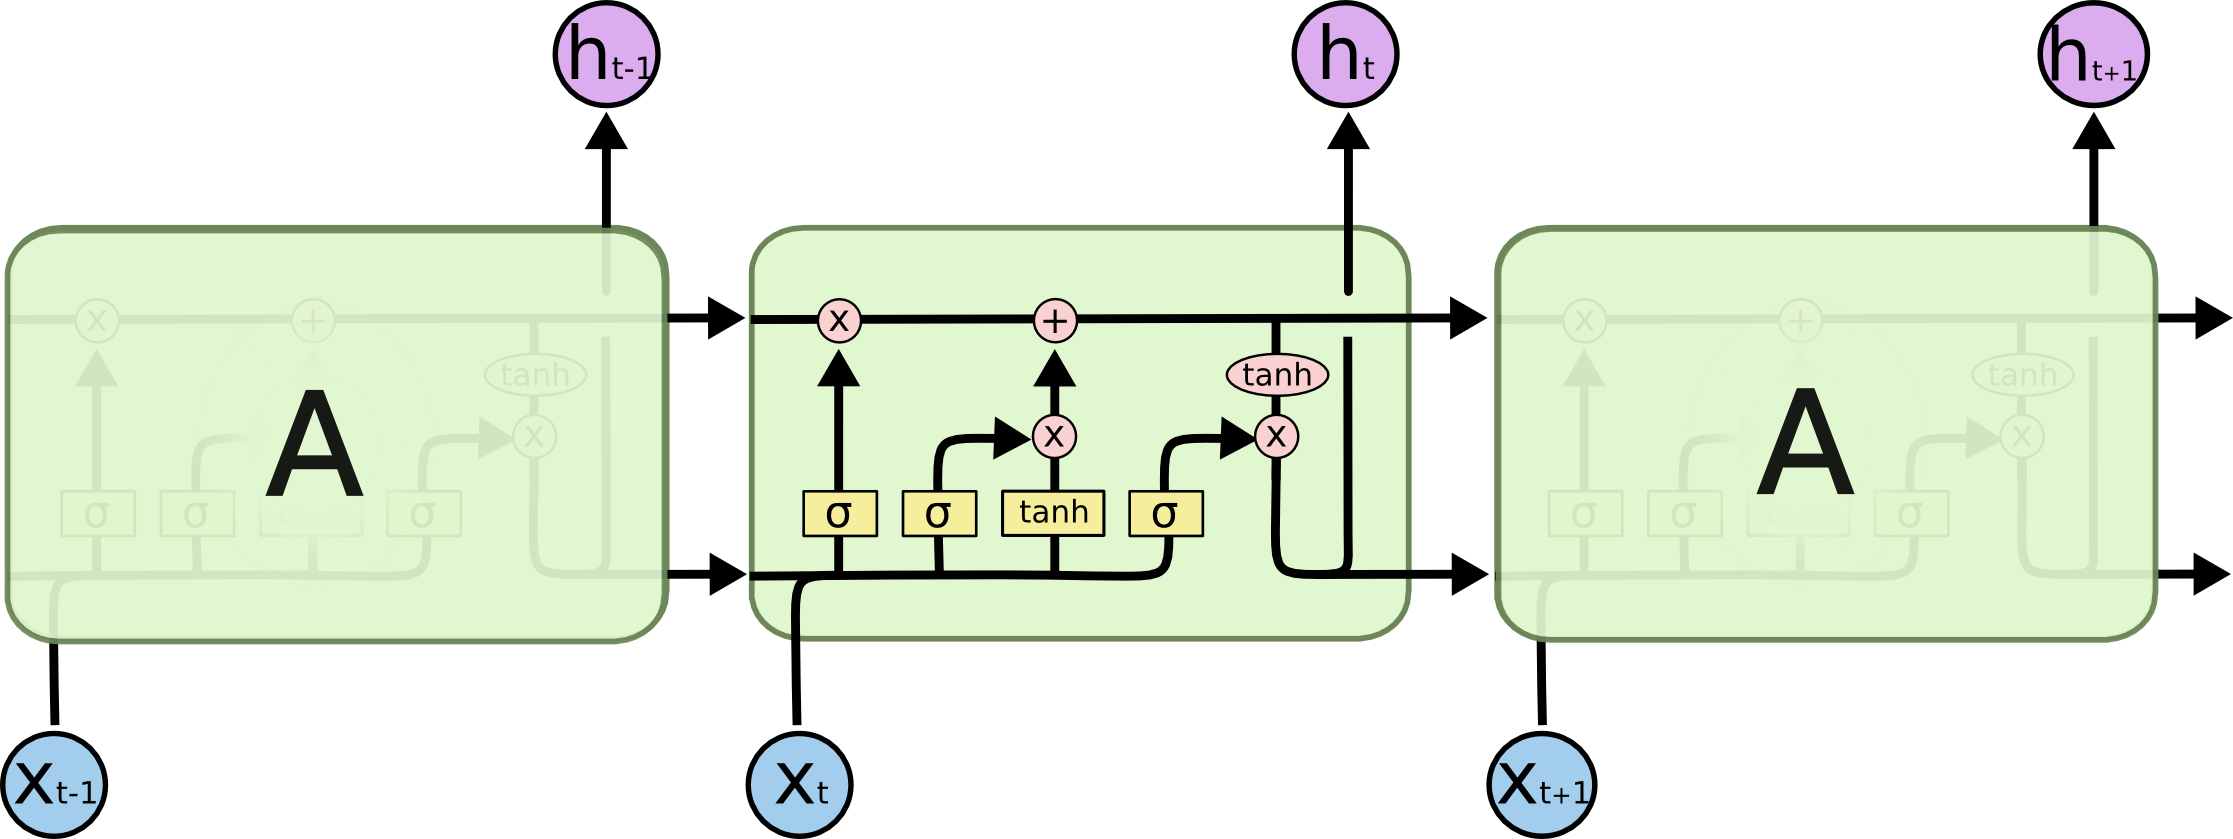
\includegraphics[width=\textwidth]{bilder/LSTM3-chain}
    \caption{Reihe von LSTM-Zellen mit entsprechenden Gates \citep{lstmexplained}}
\end{figure}

\pagebreak
